\documentclass[12pt, twoside]{article}
\usepackage[letterpaper, margin=1in, headsep=0.5in]{geometry}
\usepackage[english]{babel}
\usepackage[utf8]{inputenc}
\usepackage{amsmath}
\usepackage{amsfonts}
\usepackage{amssymb}
\usepackage{tikz}
\usepackage{yhmath}
%\usetikzlibrary{quotes, angles}

\usepackage{graphicx}
\usepackage{enumitem}
\usepackage{multicol}

\usepackage{fancyhdr}
\pagestyle{fancy}
\fancyhf{}
\renewcommand{\headrulewidth}{0pt} % disable the underline of the header

\fancyhead[RE]{\thepage}
\fancyhead[RO]{\thepage \\ Name: \hspace{3cm}}
\fancyhead[L]{BECA / Dr. Huson / 10th Grade Geometry\\* 10 May 2019}

\begin{document}
\subsubsection*{10.12 Unit Exam: Volume, density, trig, \& review}
 \begin{enumerate}

  \item Find the area of a semi-circle diameter of 10. Round your answer to the  \emph{nearest tenth}.\vspace{3cm}

  \item A cylindrical pipe with radius $r=6$ inches has a volume of $15.7$ cubic feet. Find the length of the pipe, to the \emph{nearest foot}. \vspace{3.5cm}
  \item A box in the shape of a rectangular prism must have a volume of 30 cubic feet. It's length is 4 feet and width 3 feet. How tall must it be? \vspace{3.0cm}

  \item The area of $\triangle ABC$ is $120.7$ square inches. The altitude $h$ of the triangle is 8.5 inches. Find the length of the base $AB$.\\[0.5cm]
  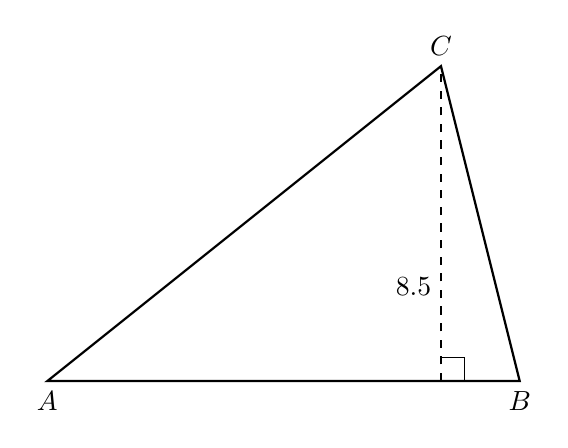
\begin{tikzpicture}[scale=1.0]
   \draw [thick]
     (0,0)node[below]{$A$}--
     (6,0)node[below]{$B$}--
     (5,4)node[above]{$C$} --cycle;
  \draw [dashed] (5,0)--(5,4);
  \draw (5,0)++(0.3,0)--++(0,0.3)--+(-0.3,0);
  \node at (5,1.2)[left]{$8.5$};
  %\node at (3,0)[below]{$20.7$};
  \end{tikzpicture} \vspace{0.5cm}

\newpage
\item Which three-dimensional figure will result when a right triangle 8 inches tall and 3 inches wide is continuously rotated about the longer side?
  \begin{enumerate}
    \item a cone with a height of 6 inches and radius of 8 inches
    \item a cone with a height of 8 inches and diameter of 6 inches
    \item a cylinder with a radius of 8 inches and a height of 6 inches
    \item a cylinder with a diameter of 6 inches and a height of 8 inches
  \end{enumerate}

  \item A right cylinder is cut perpendicular to its base. The shape of the cross section is a
    \begin{enumerate}
      \item circle
      \item cylinder
      \item rectangle
      \item triangular prism
    \end{enumerate}

  \item A bakery sells hollow chocolate spheres. The larger diameter of each sphere is 4 cm. The thickness of the chocolate of each sphere is 0.5 cm. Determine and state, to the nearest tenth of a cubic centimeter, the amount of chocolate in each hollow sphere.\\[0.5cm]
  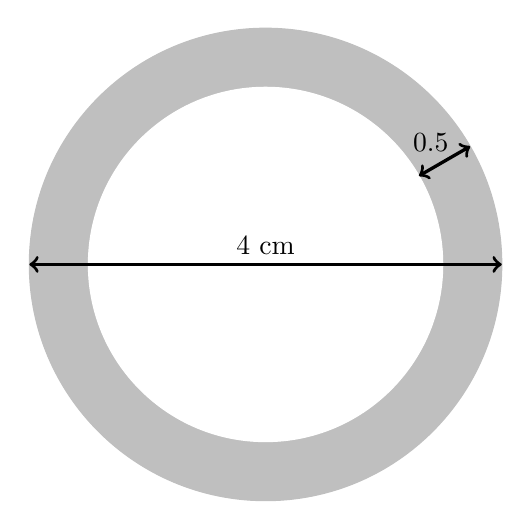
\begin{tikzpicture}[scale=1.5]
    \draw [fill, color=lightgray] (0,0) circle[radius=2];
    \draw [fill, color=white] (0,0) circle[radius=1.5];
    \draw [very thick, <->] (0:2)--(180:2);
    \draw (0,0) node[above]{$4$ cm};
    \draw [very thick, <->]  (30:1.5)--(30:2);
    \draw (32:1.65) node[above]{$0.5$};
  \end{tikzpicture}

\newpage

  \item $\triangle ABC$ is shown with $m\angle C=90^\circ$ and the lengths of the triangle's sides are $BC=8$, $AC=6$, and $AB=10$.
  \begin{multicols}{2}
        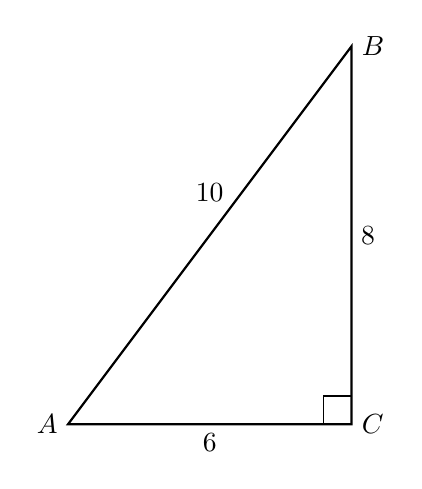
\begin{tikzpicture}[scale=0.6]
          \draw [thick]
          (0,0)node[left]{$A$}--
          (6,0)node[ right]{$C$}--
          (6,8)node[right]{$B$}--cycle;
          \draw (6,0)++(-0.6,0)--++(0,0.6)--+(0.6,0);
          \node at (3,0)[below]{$6$};
          \node at (6,4)[right]{$8$};
          \node at (3,4.5)[above]{$10$};
        \end{tikzpicture}
        \begin{enumerate}
        \item State, as a decimal, the value of $\sin A$. \vspace{0.75cm}
        \item Find the measure of $\angle A$, to the \emph{nearest degree}. \vspace{0.75cm}
        \item Find the degree measure of $\angle B$. Justify your answer.
      \end{enumerate}
    \end{multicols}
    \vspace{1.25cm}

   \item A sailor observes the top of a lighthouse with an angle of elevation of $4^\circ$. She knows the lighthouse is 100 feet tall. Determine and state the distance $x$ between the sailor and the lighthouse, to the \emph{nearest foot}.\\[0.25cm]
   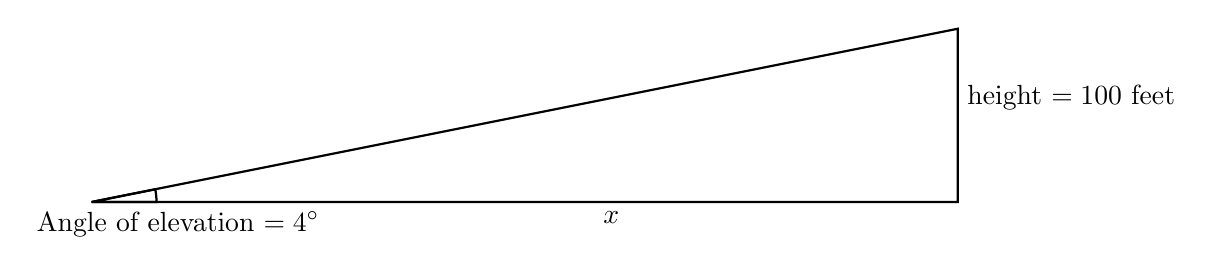
\begin{tikzpicture}[scale=1.1]
     \draw [thick] (10,0)--(0,0)--(10,2.0)--cycle;
     \draw [thick] (0,0)--(0.75,0) arc [start angle=0, end angle=11.3, radius=0.75]--cycle;
     \node at (1,0)[below]{Angle of elevation $=4^\circ$};
     \node at (10,1.2)[right]{height $=100$ feet};
     \node at (6,0)[below]{$x$};
   \end{tikzpicture} \vspace{3.25cm}

\newpage
\item   Solve for the value of $x$.\\[0.5cm]
$\frac{1}{5}(2x+3)=1$ \vspace{3cm}

\item Given $f(x)=\frac{1}{4} x+4$. Solve for $x$ such that for $f(x)=6$. \vspace{3.5cm}
\item Given $g(x)=3x^2-7x+5$. Simplify $g(0)$. \vspace{2cm}
\item Given $f(x)=5x-22$. Solve for $x$ such that for $f(x)=3$. \vspace{3.5cm}
\item Given $h(x)=x^2+6x+5$. Solve $h(x)=0$. \vspace{3cm}

\newpage
\item A translation maps $A(3,5) \rightarrow A'(-2,7)$. What is the image of $B(-4,1)$ under the same translation?  \vspace{1.5cm}

\item The line $l$ has the equation $y=-\frac{3}{5}x+4$. To each line below, circle whether $l$ is parallel, perpendicular, or neither.
  \begin{enumerate}
    \item parallel \quad perpendicular \quad neither \qquad $y=\frac{3}{5}x-2$
    \vspace{0.5cm}
    \item parallel \quad perpendicular \quad neither \qquad $3x-5y=-15$
    \vspace{2.5cm}
  \end{enumerate}

\item Simplify each expression. (Leave it in radical form if necessary, not a decimal.)
  \begin{enumerate}
    \begin{multicols}{2}
    \item   $\sqrt{20}$ \vspace{1.25cm}
    \item   $\sqrt{\frac{16}{49}}$ \vspace{1.25cm}
    \end{multicols}
  \end{enumerate} \vspace{2cm}


\item Given $m\angle R=40$ and $m\angle U=80$. Find $m\angle UST$.\\[1cm]
\begin{tikzpicture}
 %\draw [->, thick] (0,0)--(5,5);
 \draw [<-, thick] (8,0)--(0,0)--(3,3)--(4.5,0);
 \draw [fill] (0,0) circle [radius=0.05] node[below]{$R$};
 \draw [fill] (4.5,0) circle [radius=0.05] node[below]{$S$};
 \draw [fill] (3,3) circle [radius=0.05] node[right]{$U$};
 \draw [fill] (7,0) circle [radius=0.05] node[below]{$T$};
\end{tikzpicture} \vspace{1cm}

\item Write down the center and radius of each circle.
 \begin{enumerate}
   \begin{multicols}{2}
   \item   $(x-1)^2+(y+3)^2=81$ \vspace{2.5cm}
   \item   $x^2+y^2=49$ \vspace{2.5cm}
   \end{multicols}
 \end{enumerate} \vspace{2cm}

\newpage
\item In the diagram below, $\overline{AC}$ has endpoints with coordinates $A(-4, 5)$ and $C(5, 2)$.
 \begin{center} %4 quadrant regents grid
   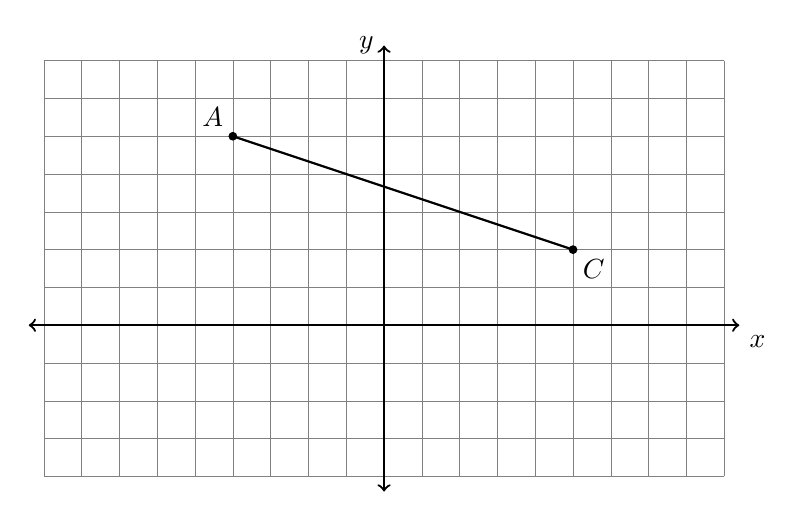
\begin{tikzpicture}[scale=.48]
     \draw [help lines] (-9,-4) grid (9,7);
     \draw [thick, <->] (-9.4,0) -- (9.4,0) node [below right] {$x$};
     \draw [thick, <->] (0,-4.4)--(0,7.4) node [left] {$y$};
     \draw [thick] (-4, 5)--(5, 2);
     \draw [fill] (-4, 5) circle [radius=0.1] node[above left] {$A$};
     \draw [fill] (5, 2) circle [radius=0.1] node[below right] {$C$};
   \end{tikzpicture}
 \end{center}
 If $B$ is a point on $\overline{AC}$ and $AB {:} BC = 1{:}2$,  what  are  the coordinates of $B$? \vspace{4cm}

\item Triangle $ABC$ is dilated with a scale factor of $k$ centered at $A$, yielding $\triangle ADE$, as shown. Given $AB=9$, $BC=12$, $AC=15$, and $DE=16$. \\[0.25cm] Find $BD$, $AE$, and $k$ (the scale factor).\\[0.25cm]
   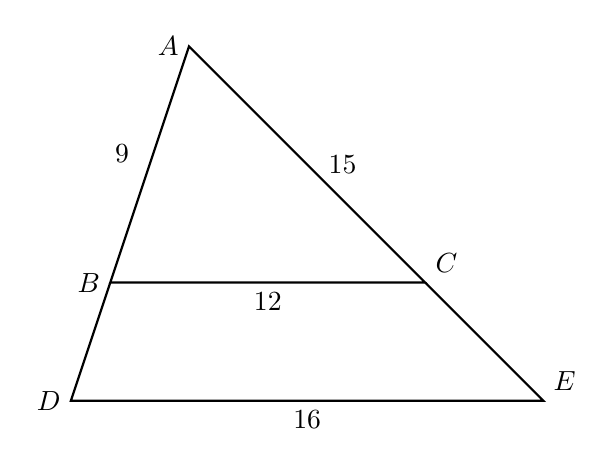
\begin{tikzpicture}[scale=0.5]
     \draw [thick]
     (0,0)node[left]{$B$}--
     (8,0)node[above right]{$C$}--
     (2,6)node[left]{$A$}--cycle;
     \draw [thick]
     (0,0)--
     (-1,-3)node[left]{$D$}--
     (11,-3)node[above right]{$E$}--(8,0);
     \node at (4,0)[below]{$12$};
     \node at (5.3, 3)[right]{$15$};
     \node at (0.3, 2.8)[above]{$9$};
     \node at (5,-3)[below]{$16$};
   \end{tikzpicture}
\vspace{2cm}

\newpage
\item What is the smallest non-zero angle of rotation about its center that would map the octagon onto itself? \vspace{0.25cm}
\begin{center}
  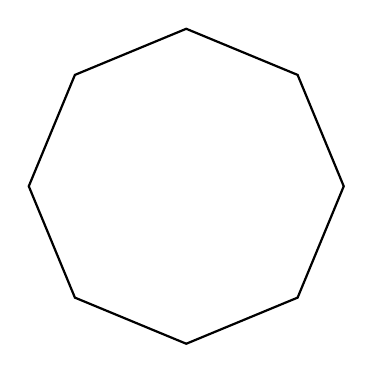
\begin{tikzpicture}%[scale=.48]
    \draw [thick]
    (0:2)--
    (45:2)--
    (90:2)--
    (135:2)--
    (180:2)--
    (225:2)--
    (270:2)--
    (315:2)--cycle;
  \end{tikzpicture}
\end{center} \vspace{2cm}

\item What transformation maps $\triangle ABC$ onto $\triangle DEF$, shown below? Fully specify the transformation.
  \begin{center}
    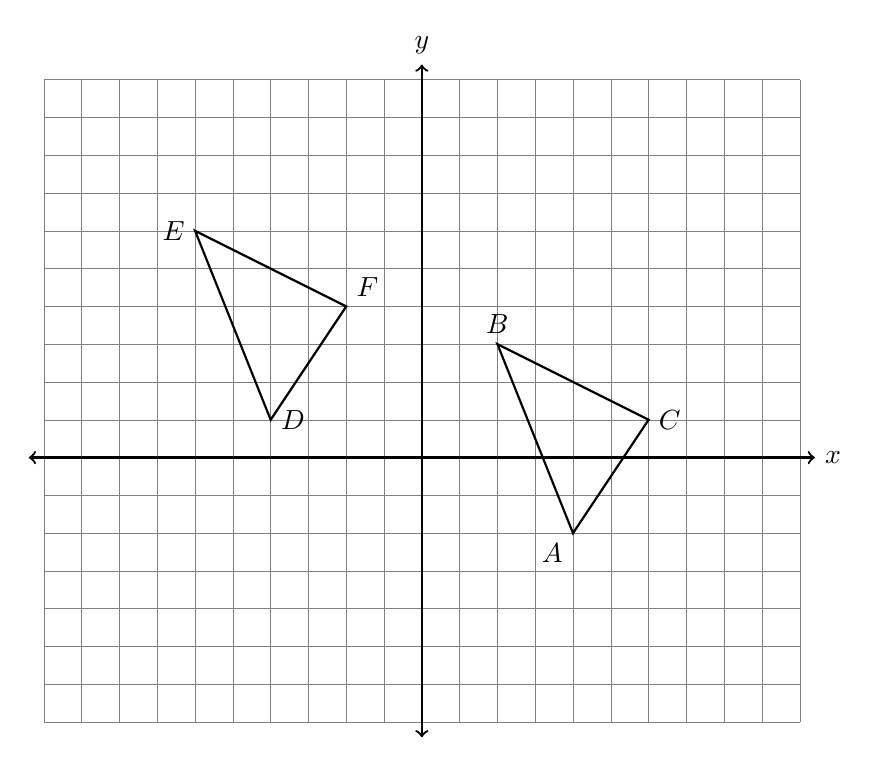
\begin{tikzpicture}[scale=.48]
      \draw [help lines] (-10,-7) grid (10,10);
      \draw [thick, <->] (-10.4,0) -- (10.4,0) node [right] {$x$};
      \draw [thick, <->] (0,-7.4)--(0,10.4) node [above] {$y$};
      \draw [thick]
        (4,-2) node[below left] {$A$}--
        (2,3) node[above] {$B$}--
        (6,1) node[right] {$C$}--cycle;
      \draw [thick]
        (-4,1) node[right] {$D$}--
        (-6,6) node[left] {$E$}--
        (-2,4) node[above right] {$F$}--cycle;
    \end{tikzpicture}
  \end{center}

\newpage
  \item In a right triangle, the acute angles have the relationship $\sin (2x)=\cos(70)$.\\[0.25cm]
    What is the value of x? \vspace{2.5cm}

  \item If $\sin (8x-8)^\circ = \cos(7x+8)^\circ$, what is the value of $x$? \vspace{3cm}

  \item Write an equation of the line that is perpendicular to the line whose equation is $3y=2x+6$ and passes through the point $(-1,7)$. \vspace{2cm}

  \item Find the distance between $(1,9)$ and $(6, -3)$.



\newpage
  \item The secants $\overline{ABC}$ and $\overline{ADE}$ intersect the circle $O$, as shown in the diagram. \\Given $m \wideparen{BD}=30^\circ$ and $m \wideparen{CE}=150^\circ$. Find the $m\angle A$.
       \begin{center}
       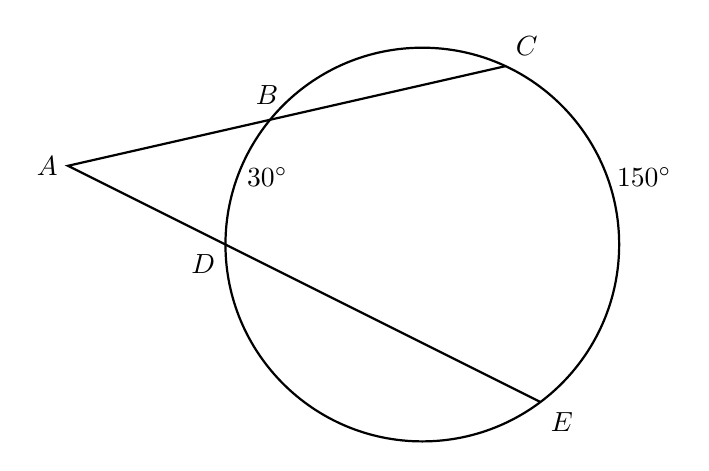
\begin{tikzpicture}[scale=.5]
         \draw [thick] (0,0) circle[radius=5];
         \draw [thick]
         (3,-4) node[below right] {$E$}--
         (-5,0) node[below left] {$D$}--
         (-9,2) node[left] {$A$}--
         (65:5) node[above right] {$C$};
         \draw (132:5.1) node[left] {$B$};
         \draw (20:5) node[right] {$150^\circ$};
         \draw (160:5) node[right] {$30^\circ$};
       \end{tikzpicture}
     \end{center} \vspace{2cm}

   \item Given circle $Z$ with inscribed $\triangle XYZ$. $m\angle Z=100$. Find $m\angle Y$.\\[1cm]
       %\hspace{1cm} Given the line  $l$ and point $P$.
       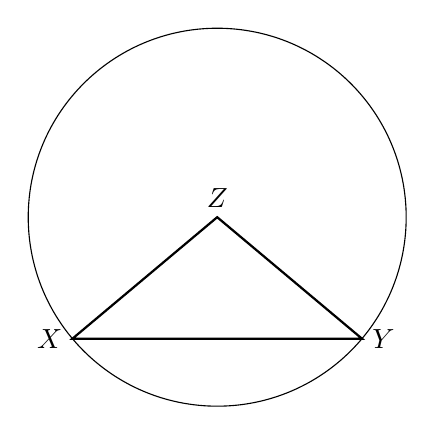
\begin{tikzpicture}[scale=0.8]
         %\draw [-, thick] (-6,0) node[left]{$A$}--(0,0);
         \draw  (0,0) circle [radius=3] node[above]{$Z$};
         \draw [-, thick] (220:3) node[left]{$X$}--(0,0)
           --(320:3) node[right]{$Y$}--cycle;
         %\node at (8.5,-0.4){$l$};
         %\draw [fill] (6,0) circle [radius=0.05] node[below]{$Q$};
       \end{tikzpicture} \vspace{3cm}

\newpage
\subsubsection*{Early finishers}

  \item A monument in the shape of a pyramid with a square base has a volume of 24 cubic feet. If its height measures 20 feet what is the length of the side of the base, to the \emph{nearest cubic foot}? \vspace{3.5cm}


  \item A staircase riser is cut as a series of congruent triangles with each step's ``rise" equal to 8 inches, and the ``run" of each step is 10 inches, as shown below. ($AB=8$ and $BC=10$) Find the diagonal length of the two-step riser, the distance $AE$, to the \emph{nearest inch}.\\[0.5cm]
        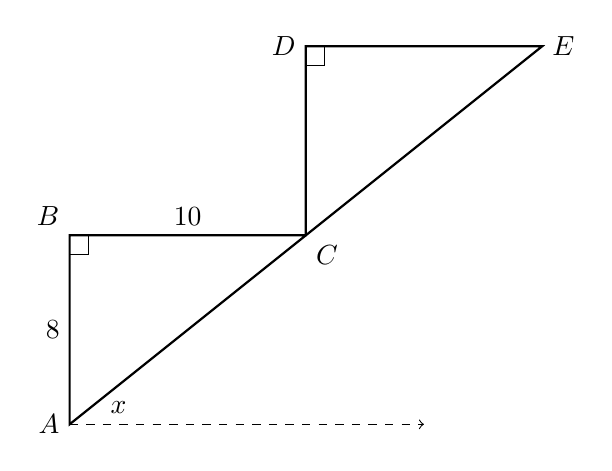
\begin{tikzpicture}[scale=0.3]
          \draw [thick]
          (0,0)node[left]{$A$}--
          (0,8)node[above left]{$B$}--
          (10,8)node[below right]{$C$}--
          (10,16)node[left]{$D$}--
          (20,16)node[right]{$E$}--cycle;
          \draw [dashed, ->] (0,0)--(15,0);
          \draw (0,8)++(0,-0.8)--++(0.8,0)--+(0,0.8);
          \draw (10,16)++(0,-0.8)--++(0.8,0)--+(0,0.8);
          \node at (0,4)[left]{$8$};
          \node at (5,8)[above]{$10$};
          \node at (28:1.5)[right]{$x$};
        \end{tikzpicture}\\
      What is the angle of inclination of the staircase, $x$?

   \item Given circle $O$ with inscribed $\triangle SLO$. $m\angle S=x+7$. Find $m\angle O=2x-2$. Find $x$.\\
   For full credit, check your answer.\\[1cm]
       %\hspace{1cm} Given the line  $l$ and point $P$.
       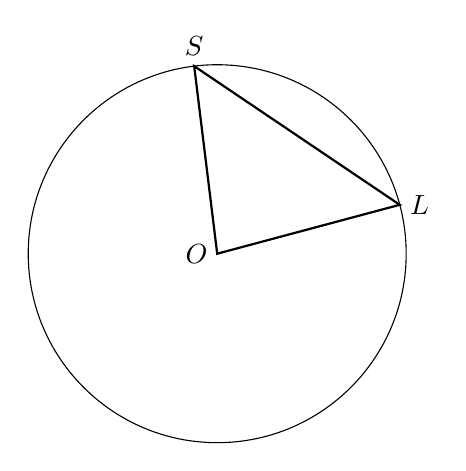
\begin{tikzpicture}[scale=0.8]
         %\draw [-, thick] (-6,0) node[left]{$A$}--(0,0);
         \draw  (0,0) circle [radius=3] node[left]{$O$};
         \draw [-, thick] (15:3) node[right]{$L$}--(0,0)
           --(97:3) node[above]{$S$}--cycle;
         %\node at (8.5,-0.4){$l$};
         %\draw [fill] (6,0) circle [radius=0.05] node[below]{$Q$};
       \end{tikzpicture}

\newpage
   \item From a point on the ground one-half mile from the base of a historic monument, the angle of elevation to its top is $11.87^\circ$. To the nearest foot, what is the height of the monument?\\[1cm]
    \begin{tikzpicture}[scale=1.1]
      \draw [dashed] (10,0)--(0,0)--(10,2);
      \draw [thick, ->] (10,0)--(10,2);
      \draw (10,0)++(-0.3,0)--++(0,0.3)--+(0.3,0);
      \fill [gray] (0,0)--(0.75,0) arc [start angle=0, end angle=11.3, radius=0.75]--cycle;
      \node at (1,0)[below]{$11.87^\circ$};
      \node at (10,1)[right]{Monument};
      \node at (6,0)[below]{One-half mile};
    \end{tikzpicture} \vspace{3cm}

   \item A homeowner is building three steps leading to a deck, as modeled by the diagram below. All three step rises, $\overline{HA}$,  $\overline{FG}$, and  $\overline{DE}$, are congruent, and all three step runs, $\overline{HG}$,  $\overline{FE}$, and  $\overline{DC}$, are congruent. Each step rise is perpendicular to the step run it joins. The measure of $\angle CAB = 36^\circ$ and $\angle CBA = 90^\circ$.\\[0.5cm]
     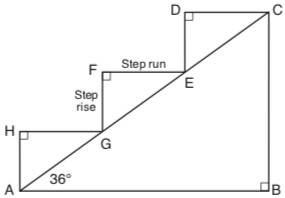
\includegraphics[width=0.4\textwidth]{steps_Aug2018-33.png}\\
   If each step run is parallel to $\overline{AB}$ and has a length of 10 inches, determine and state the length of each step rise, to the \emph{nearest tenth of an inch}.\\[3cm]
   Determine and state the length of $\overline{AC}$, to the \emph{nearest inch}.

   \item The secants $\overline{PQR}$ and $\overline{PST}$ intersect the circle $O$, as shown in the diagram. \\Given $m \angle P=40^\circ$ and $m \wideparen{RT}=140^\circ$. Find the $m\wideparen{QS}$.
        \begin{center}
        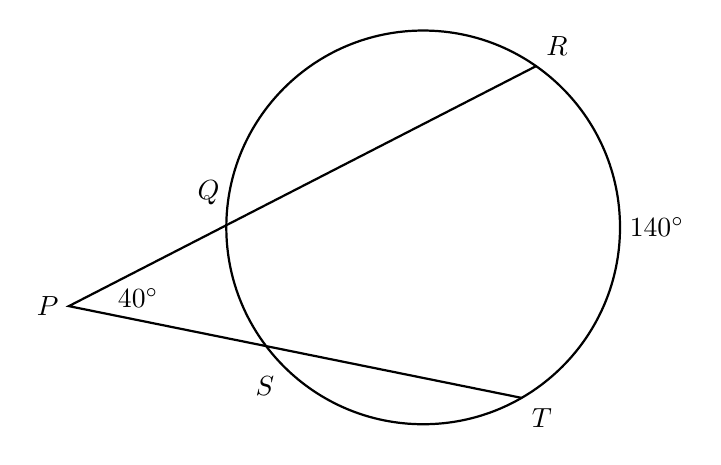
\begin{tikzpicture}[scale=.5]
          \draw [thick] (0,0) circle[radius=5];
          \draw [thick]
          (-60:5) node[below right]{$T$}--
          (-9,-2) node[left]{$P$}--
          (55:5) node[above right]{$R$};
          \draw (225:5) node[below left]{$S$};
          \draw (170:5) node[left] {$Q$};
          \draw (0:5) node[right] {$140^\circ$};
          \draw (-8,-1.8) node[right] {$40^\circ$};
        \end{tikzpicture}
      \end{center} \vspace{1cm}


\end{enumerate}
\end{document}


   \item On the set of axes below, $\triangle ABC$, altitude $\overline{GC}$, and  median $\overline{MC}$ are drawn.
    \begin{center}
      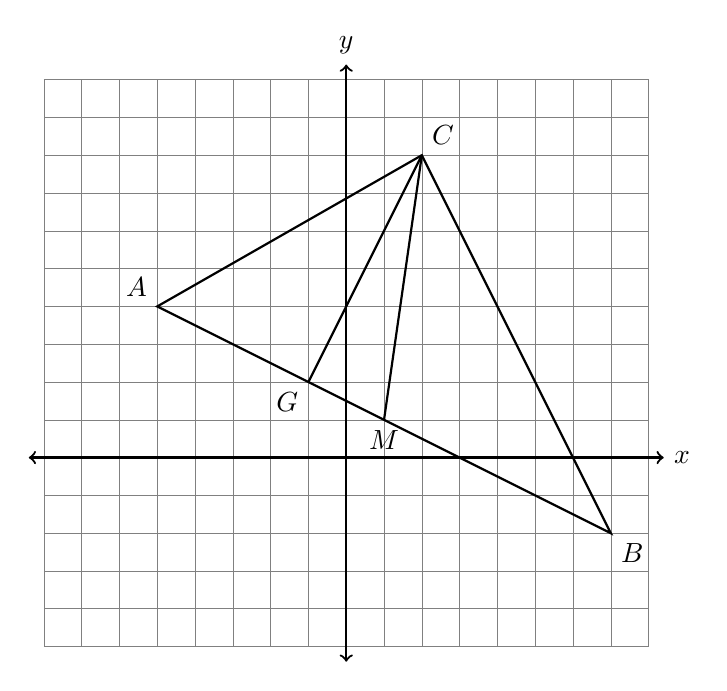
\begin{tikzpicture}[scale=.48]
        \draw [help lines] (-8,-5) grid (8,10);
        \draw [thick, <->] (-8.4,0) -- (8.4,0) node [right] {$x$};
        \draw [thick, <->] (0,-5.4)--(0,10.4) node [above] {$y$};
        \draw [thick]
          (-5,4) node[above left] {$A$}--
          (7,-2) node[below right] {$B$}--
          (2,8) node[above right] {$C$}--
          cycle;
        \draw [thick] (1,1) node[below] {$M$}--(2,8);
        \draw [thick] (-1,2) node[below left] {$G$}--(2,8);
      \end{tikzpicture}
    \end{center}
      Determine which equations represent the area of the triangle, circling True or False.
      \begin{multicols}{2}
       \begin{enumerate}
       \item \quad T \quad F \quad $\displaystyle Area_\triangle = \frac{(AC)(AB)}{2}$ \vspace{0.25cm}
       \item \quad T \quad F \quad $\displaystyle Area_\triangle = \frac{(CG)(BC)}{2}$
       \item \quad T \quad F \quad $\displaystyle Area_\triangle = \frac{(CM)(AB)}{2}$ \vspace{0.25cm}
       \item \quad T \quad F \quad $\displaystyle Area_\triangle = \frac{(CG)(AB)}{2}$
      \end{enumerate}
      \end{multicols}
      \vspace{0.25cm}


        \item The map of a campground is shown below. Campsite C, first aid station F, and supply station S lie along a straight path. The path from the supply station to the tower, T, is perpendicular to the path from the supply station to the campsite. The length of path FS is 400 feet. The angle formed by path TF and path FS is $72^\circ$. The angle formed by path   and path CS is $55^\circ$.\\[0.5cm]
        \includegraphics[width=0.5\textwidth]{camp_Jun2018-31.png}
          \begin{enumerate}
            \item Determine and state the volume of concrete needed, \emph{in cubic feet}. \vspace{1cm}
            \item Sarah can mix her own concrete for \$3.25 per cubic foot. How much money will it cost her to replace the two concrete sections?
        \end{enumerate} \vspace{2.5cm}
